\documentclass[]{UCD_CS_FYP_Report}
	\usepackage{graphicx}
	\usepackage{hyperref}
	\usepackage{cite}
	\usepackage{float}
	\usepackage{amsthm,amssymb}
	\usepackage{amsmath}
	\usepackage{algorithm}
	\usepackage[noend]{algpseudocode}
	
	%%%%%%%%%%%%%%%%%%%%%%
	%%% Input project details

	\def\studentname{Sukrat Kashyap} % Edit with your name
	\def\projecttitle{Automated Software to Understand Functional Relationship Between Dynamic Energy and Performance Events} % Edit with you project title
	\def\supervisorname{Ravindranath Reddy Manumachu}

\begin{document}
\maketitle

%%%%%%%%%%%%%%%%%%%%%%
%%% Your Project Specification

\chapter*{Project Specification}
\textbf{General Information:}

A energy model representing a relationship between dynamic energy consumption and performance events (PMCs) is constructed experimentally and the experimental dataset has the following format typically (k events, n records):

\(E_1,\ x_{11},\ x_{12},\ x_{13} \ldots x_{1k}\)\\
\(E_1,\ x_{21},\ x_{22},\ x_{23} \ldots x_{2k}\)\\
\ldots \\
\(E_n,\ x_{n1},\ x_{n2},\ x_{n3} \ldots x_{nk}\)

where \(E_i\) is the experimentally obtained dynamic energy consumption of i-th record and xij are the experimentally obtained performance events (PMCs).

Given such an experimental dataset as an input, the goal is to determine/understand the functional relationship between the dynamic energy consumption and performance events (PMCs).

Two real-life datasets will be provided to the student.\\
\textbf{Core:}

The goal is to write automated software that will detect the following:
\begin{enumerate}
    \item Existence of records where the dynamic energy consumption is the same (within an input tolerance) but all PMCs (with the exception of one) have same values. Then the relationship between energy and the one PMC is visualized to see the nature of the functional relationship.
    \item Having accomplished step (1), understand the monotonicity of the relationship between dynamic energy consumption and performance events (PMCs).
    \item Existence of records where the dynamic energy consumptions are different (within an input tolerance) but all PMCs have same values (within an input tolerance) suggesting the non-existence of a functional relationship.
\end{enumerate}

The software must be written using any one mainstream language but preferably one of the following:
C, C++, Python

The software must be well documented and tested.

\textbf{Advanced:}

Given an experimental energy model dataset as an input, the goal is to write software that performs intelligent but computationally feasible simulations where combinations of inputs are generated to study the existence/non-existence of a functional relationship between dynamic energy consumption and PMCs.

The software must be written using any one mainstream language but preferably one of the following:
C, C++, Python.

The software must be well documented and tested.

%%%%%%%%%%%%%%%%%%%%%%
%%% Your Abstract here

\begin{abstract}
	With the advent of computers, data has become the new gold in the market. Most of the companies are driven by data as storage of data is no longer a expensive commodity. But new challenges have arised due to this and everyone now is focusing on analysis of data to predict, to minimize cost or to get new relations. This project tackles one aspect of data analysis that is the existence of a mathematical functional relationship of a data. It is as simple as saying true or false meaning relationship may exit or proving the non existense of functional relationship respectively.
\end{abstract}
\newpage

%%%%%%%%%%%%%%%%%%%%%%
%%% Acknowledgments

\chapter*{Acknowledgments}
I would like to thank my supervisor Ravindranath Reddy Manumachu and mentor Alexey Lastovetsky for the assistance and guidance of this project. I would also like to thank my family and friends for supporting me in my work.

%%%%%%%%%%%%%%%%%%%%%%
%%% Table of Content

\tableofcontents\pdfbookmark[0]{Table of Contents}{toc}\newpage
\newpage

%%%%%%%%%%%%%%%%%%%%%%
%%% Introduction

\chapter{Introduction}
\section{Motivation}
Modern day technology has developed under incredible speed in recent decade and the computing power growth rate is truly phenomenal and lasting impact can be felt and benefit us in many ways. It is important to realise the worldwide effect on environment by the increase in consumption of power by these technology advancements.

According to~\cite{pickavet2008worldwide}, the power consumption growth rates of PCs are about 7.5\% per year. Data Centres and network play much larger role as they both have power consumption rate of 12\% each. This considerable growth is due to increasing data to be accessed, stored and processed. This constant expansion of energy consumption leads to increase in carbon emissions. \(CO_2\) emissions from ICT (Information and communications technology) are increasing at a rate of 6\% per year, at such rate by 2020 it will account to 12\% of worldwide emissions ~\cite{rong2016optimizing}.

\begin{figure}[ht]
	\centering
	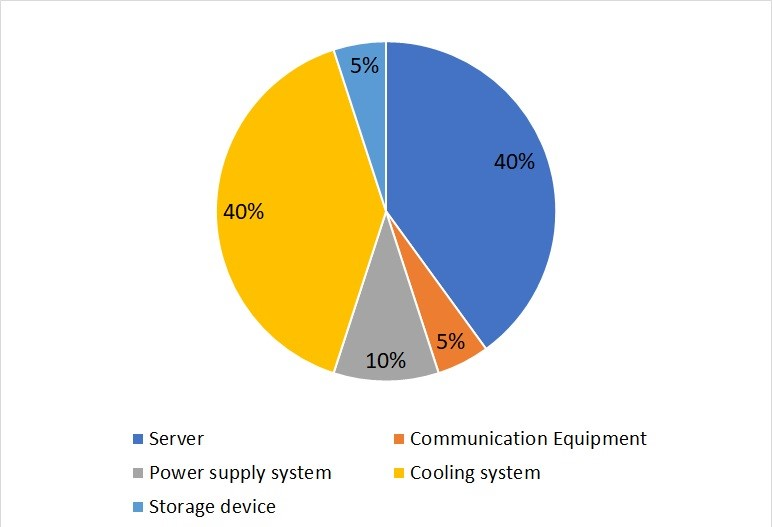
\includegraphics[width=200pt]{energypiechart}
	\caption{\label{fig:energypie} Energy consumption distribution of data centers.}
\end{figure}

The major roles of power consumption by a data ware house is played by the servers and the cooling system which is used to cool down the server physical parts. From the figure~\ref{fig:energypie}, you can see they both account to 80\% of the total consumption with both accounting for 40\% each~\cite{rong2016optimizing}. Hence by finding a relation between different events and energy consumption, we could minimize the power consumption by the systems. Minimising energy consumed will also decrease the heat generated by the system which will in turn lower down the usage of cooling system. Leading us to minimise cost and save environment.

Thus, if we could discover the functional relational between the demand of the power and the performance events (PMCs), that could enable us the ability to adjust, and predict the energy consumption for certain computations.

\section{Aims}

The projects aim is to create a piece of software that is extensible, easy to use and performant. A tool that can perform analyses like regression and clustering and give us an overview of the data by show casing the relationship of various parameters with the output. In this case, our parameters are the performance events and output is the energy consumption. Following are the objectives that we want to achieve.

\subsection{Existence of functional relation}

Datasets are mostly pair of multiple inputs and a single output. And the possibility of the existence is what we are interested in. Is it possible to define the data in a form of function? Question like this is one of the aims. Defining the data in a form of function is explaining the dataset in a form of a formula which can combine various parts of the input parameters and give the output. It is quite impossible to tell that whether a function definetly exists as the data we have is always a subset and there are number of records which are either not in the dataset or we donot know. But, regardless we can definitely explain the non-existence of a formula by finding a pair of input parameters and outputs that violate the definition of a function.

The pair which violates the definition of a function must be looked at as there is high probability of that data set record being corrupt or if not it can actually help and tell the non existence. If this outlier is in fact corrupt, this process can be used for data cleanups as well.

\subsection{Analysis of functional relation}

Once, we are no more able to prove functional non existence in the dataset. We can try to analyse the dataset and try to examine the various relations of the parameters with the output. Analysis of the parameters with output is done to know how much change in one parameter contributes to the change in the output. This analysis helps us to understand the correlation between two quantities. Does high page faults correlates to high energy consumption? Questions like this is what the analysis of parameters with their corresponding output answers. This can also be thought of an explaination of the output parameters.

In other words, understanding the correlation is the other aim. Once we are able to know that there is high correlation. We can then dig deep into the data and try to find out the reason for the same.

\section{Approach}

For each of the aims, two approaches have been employed. Both the approaches tries to achieve the same conclusions with different methodology.

The experimental data sets provided has the following format:

\(E_1,\ x_{11},\ x_{12},\ x_{13} \ldots x_{1k}\)\\
\(E_1,\ x_{21},\ x_{22},\ x_{23} \ldots x_{2k}\)\\
\ldots \\
\(E_n,\ x_{n1},\ x_{n2},\ x_{n3} \ldots x_{nk}\)

where \(k\) is the total number of parameters (performance events), \(n\) is the number of records in the dataset.
\(E_i\) is the experimentally obtained dynamic energy consumption and \(x_{ij}\) are the experimentally obtained performance events (PMCs).

\subsection{Existence of functional relation}

Our main goal here is to find nonexistence of functional relationship. In other words, it means proving that the dataset cannot be explained in terms of a function/formula.

Our first approach here is to find two performance events tuples \((x_{i1},\ x_{i2},\ x_{i3} \ldots x_{ik})\) and \((x_{j1},\ x_{j2},\ x_{j3} \ldots x_{jk})\) are equal within some tolerance, but their corresponding \(E_i\) and \(E_j\) dynamic energy consumption is different. Existence of such a tuple in database will lead us to prove the non-existence of a functional relationship.

It is infact easier to find two equal records by ordering the dataset by their parameters and going through the entire dataset once to find equal records and comparing their dynamic energy consumption. The order of complexity is O(N log N) which is the complexity of sorting as that is the only heavy duty task involved. But it gets really complicated when tolerance comes into play. In other words, we have to find similar records than equal records. The project employs 2 methods to measure the similarity between the two data records.

First approach:

The data records are imagined as data points in \(k-space\) as we have \(k\) number of parameters. Then we divide the whole space into small \(k-dimension cubes\) whose dimensions \((t_1, t_2, \ldots t_k)\) where \(t_i\) is the tolerance of each parameter. The data points are then put in their respective cubes. And each cube is then analysed to see that whether the data points output are similar to each other as well.

Second approach:

The data points in \(k-space\) are similar if the euclidean distance between them is less than the \(t\) provided, where \(t\) is the total/max tolerance. Data points which are infact found to be close to each other, their output is compared to see if they are similar to each other.

\subsection{Analysis of functional relation}

Many different type of relations can be there between two variables. But, we are interested in more general trend of the dynamic energy consumption output with the performance events. Many researches have used linear models, to understand the relation between energy consumption and performance events.\cite{o2017survey} And this is due to the trickle down effect of the relation.\cite{bircher2007complete} Hence, we also used linear regression to analyse the relationship.

Linear regression is done with 2 variables but we have \(k\) variables relation to energy consumption making it hard to understand the nature. Hence to analyse one of the variable we have to isolate it in the space where the other \(k-1\) variables donot change. Data points are clustered using \(k-1\) variables. Each cluster is then visited and linear regression is performed. Two approaches are employed to cluster which are similar to finding similar records in finding the existence of the relation.

First approach:

Data points are clustered by putting the data points in the respective \(k-1 dimension cube\). Forming a cluster with almost similar \(k-1 variables\).

Second approach:

Euclidean distance is used to isolate similar \(k-1 variables\). A \(k-1 dimension sphere\) can be imagined for simplicity with its radius being the total/max tolerance.

In both approaches, linear regression is performed on the cluster with the variable which was not used in clustering and the output which is the dynamic energy consumption.

Above is just only one field that possible usage of the functional relationship in data. In real world there are much more application that required such technique. Such as hybrid vehicle power management, power supply of auxiliary power units etc. There are many past work in this field but only few were focus on the relationship between dynamic energy consumption and PMCs. Hence, in this report we will try to observe the relationship between energy consumption and PMCs. We will explore the monotonicity of the relationship between dynamic energy consumption and performance events (PMCs) and suggesting the non-existence of a functional relationship as well.

\section{Structure of report}
In this report, you must have already seen the motivation behind the project and brief description of the approaches that will be taken to reach the objective.

This Introductory chapter is followed by Background research, design aspects of the software, implementation of the software, testing and evaluation of the tool followed by the conclusion and the future works.

Background research explains about performance events and how do they influence energy consumption by the system. It also explains the approaches in detail mentioned above and analyses their complexity and how they can be optimised.

Following Background research, design and implementation of the software is deep dig into as we want an extensible, performant tool. Testing and evaluation of the software is explained. How the software is tested and its evaluation on its performance. The report ends with conclusions and future works that shows how the project can be extended and applied to various other domains.

%%%%%%%%%%%%%%%%%%%%%%
%%% Background Research

\chapter{Background Research}
Many designers are increasingly utilizing dynamic hardware adaptations to improve performance while limiting the power consumption. Whereas Some are using software to decrease power usage for e.g. putting the system in sleep mode when it's in the idle state. The main goal remains the same, which is to extract maximum performance while minimizing the temperature and power. The study and examination of the events affecting the consumption will help us to predict and minimize the consumption of energy with very high accuracy.

\section{Energy consumption and Performance Events}

First, let's look at energy consumption. Energy consumption is the power (usually in watts) consumed by a system. This system could be the processor/CPU, memory, disk, I/O (Input/Output) system, chipset or the whole computer system itself. It has been known that power consumption of any system has a high correlation to its usage. Since the correlation is high for its usage. It means usage is a is a good way to understand the power consumption. Performance events are one of the better ways to measure the usage of a system as they are known much more faster than the temperature sensors. As temperature sensors are slow in response due to the thermal inertia of the microprocessor.

Now let's look at what are performance events, performance events are any events that affect the consumption of energy in some way. Selection of performance events is quite challenging. A simple example would be the effect of cache misses in the processor. For a typical processor, the highest level of cache would be L3 or L2 depending on the type of processor. Now for some transaction which could not be found in the highest level of cache (cache miss) would cause a cache block size access to the main memory. Thus, the number of main memory access would be directly proportional to the cache misses. Since this memory access is off-chip, power is consumed in the memory controller and DRAM. Even though, the relation is not simple as it seems but a strong casual linear relationship between the cache miss and the main memory power consumption~\cite{bircher2007complete}.

Another performance event can be instructions executed. The more instruction being executed, will turn on and use more units of the system. Hence, power is consumed as opposed to when the processor is in its idle state~\cite{gilberto2005power}.

Cache miss, TLB misses are also good performance events as they seem to have a strong relationship between the power consumption as processor needs to handle memory page walks. Same can be said for Page faults where a program is not able to find mapped address in physical memory as it has not been loaded yet. This causes a trap which can result in a number of situations, one of them which is to get the data from disk. It involves a long walk to the disk. This walk to the disk and raising of exceptions would consume more energy by the disk as well as the CPU. Another thing to note here most of the relations that we saw above are directly proportional to each other. Increase in the variable like cache miss, the number of cycles in CPU etc gives rise to energy consumption by the system. This makes a linear model a good point to start when analysing the relationship between the performance events variables and energy consumption.

\section{Related Work}

In this section, some of the prior research are discussed. Hardware performance counter's links to processor power consumption were first demonstrated by Bellosa. In \cite{bellosa2000benefits}, Bellosa demonstrated the high correlation between performance counters such as memory references, L2 cache, floating point operations to processor power consumption.

Gilbert in \cite{gilberto2005power}, predicted the power consumption for Intel XScale processors using performance monitoring unit events. Since power consumption is greatly dependent on executing workload, power estimation was done using HPCs (Hardware performance counters) such as Instruction cache miss, TLB misses etc. The linear parameterisation of power consumption based on performance events was done based on performance events. 

In \cite{yang2016performance}, proposed a full system power model for CPU-intensive and memory intensive applications with active cycles, instruction retired and LLC missed as performance events. A full power model for I/O intensive applications was also proposed considering the system level utilization as performance events. Many machine learning based algorithms like logistic regression, elastic net and k-nearest neighbours were applied to the real-world application. 

Bircher approached in a distinct way by using events local to the processor and eliminating the need for sensors spread across various parts of the systems \cite{bircher2012complete}. Linear regression modelling was done in order to predict the power consumption at runtime. Multiple linear and polynomial regression was done only when accuracy was not obtained. 

The high correlation between performance events and power consumption was demonstrated by all of them. But all of them tried to predict the power consumption using system events. They use various methodologies in predicting so. In \cite{yang2016performance}, a number of machine learning algorithms were used. But in this project, an attempt is made to understand the monotonic relation between the events and power. The predictive models would work on a particular specification of the system. But understanding the relation will help define a model on the architecture level. This will also help in verifying the models that already exist.


\section{Existence of functional relation}

\textbf{Definition}: \textit{Given a dataset of pairs \((x_i, y_i)\) where \(i \in [1, n]\) of two variables \(x\) and \(y\), and the range \(X\) of \(x\), \(y\) is a function of \(x\) iff for each \(x_0 \in X\), there is exactly one value of \(y\), say \(y_0\), such that \((x_0, y_0)\) is in dataset.}~\cite{zembowicz1993testing}

Above is the definition of functional relation. In our case the \(x_i = (p_1, p_2, \ldots p_k)\) and \(y_i = E_i\) where \(p\) are the performance events and \(k\) is the number of events and \(E\) is the energy consumption.

In other words, functional relationship is an one to one mapping between our input variables \(p_1, p_2, \ldots p_k\) and output \(E_i\). This reasoning can be explained quite intuitively as assuming functional relation we can formulate a \(f(p_1, p_2, \ldots p_k) = E_i\) where \(f\) is function. Now if one \((p_1, p_2, \ldots p_k)\) can give more than one output \(E_i\) then that \(f\) function is either not correct or \(f\) does not exist. A question that immediately arises is what if two different \((p_1, p_2, \ldots p_k)\) gives same output \(E_i\). The answer is it is possible and it does not violate the functional relation definition as there is still 1 to 1 mapping from input to output. The only difference is the functional relation is not surjective anymore which means that one cannot figure out the input values from output values (i.e. the other way around). But we are only interested in predicting the output rather than inputs from the output variables.

The Proof of the existence of functional relation is given below:

But first, let's look at our dataset that will be provided.
We know that the data will be in the following format:

Let \(k\) be the number of parameters for the energy and \(n\) be the number of records in the dataset

\(E_1,\ x_{11},\ x_{12},\ \ldots x_{1k}\)\\
\(E_2,\ x_{21},\ x_{22},\ \ldots x_{2k}\)\\
\ldots\\
\(E_n,\ x_{n1},\ x_{n2},\ \ldots x_{nk}\)\\
where \(E_n\) is the dynamic energy for the nth tuple and \(x_{nk}\) corresponds to the \(k\)th performance event for \(n\)th record.

We will use mathematical definition of functional relationship given above to prove the approaches:

\textbf{To Prove:} We need to prove that finding at least 2 equal performance events with different dynamic energies ensures that there exists no functional relationship in the dataset.

\begin{proof}
    Let us assume that there exists a functional relation such that:\\
    \(f(x_{n1},\ x_{n2},\ \ldots x_{nk}) = E_n\)\\
    where \(f\) is the functional relation for the dataset.

    If we have \(f(x_{i1},\ x_{i2},\ \ldots x_{ik}) = E_i\) and \(f(x_{j1},\ x_{j2},\ \ldots x_{jk}) = E_j\)
    where \(E_i \neq E_j\) and \((x_{i1},\ x_{i2},\ \ldots x_{ik}) = (x_{j1},\ x_{j2},\ \ldots x_{jk})\)

    If such \(i\) and \(j\) exists. Then, we can conclude that the \(f\) is not a function by using the definition of a function as this assumed function has two images.

    Which contradicts the hypothesis stated above.
    Hence by proof of contradiction, we could say that \(f\) is not a function of the dataset.
\end{proof}

Now the task is to find similar \(x_{11},\ x_{12},\ \ldots x_{1k}\) input variables. If it was equality, it could be performed trivially by sorting the data records on the basis of \(x_{11},\ x_{12},\ \ldots x_{1k}\). Followed by going through the data records in that order to find equal records. As equal records will be next to each other when sorted.

But the dataset accumulated is collected from experimental setup. Experimental setups data have some error/tolerance associated with it. As the equipment or software cannot accurately measure and have some error associated with it. e.g. Energy consumption is measured by a power meter which does have a confidence interval. The tolerance associated with the dataset no longer allows performing equality on input variables. Hence, a method is needed to measure the equality of the tolerance.

Now after knowing the tolerances the data records in the dataset now looks more of the form:

\(E_n \pm e_E,\ x_{n1} \pm e_1,\ x_{n2} \pm e_2,\ \ldots x_{nk} \pm e_n\)\\
where \(e\) is now the error associated with the variable.

Hence dataset must be clustered with the tolerances associated with them. Data points having similar \(k\) parameters will fall in the same cluster. The output variable \(E_n \pm e_E\) must be close to each other within some tolerance for all the points in the cluster. If they are not, it violates the functional relation and the data points are picked and must be given to the user to either discard if corrupt. This removal of corrupt data records is known as Data cleanups. If they are not corrupt then it proves the non-functional relation in the dataset. Analysis of functional relation can be done when no records are found that contradicts the functional relation definition.

\section{Analysing functional relation}

Now this section corresponds to analysing the functional relation. A functional relation can of many forms, there can be logarithmic functional relation, exponential, linear, polynomial etc. According to \cite{bircher2007complete}, shows that functional relation between performance event and dynamic energy is of the linear form. This is due to the trickle-down effect of the performance events. Hence, Linear model is used to understand the relationship between the events and the consumption. 

This project is more interested in finding whether a strong relation of monotonicity exists in the dataset or not. And linear regression is best suited for this kind of task. Linear regression is an approach determine how strongly two variables correlate with each other. Correlation does not necessarily mean causation. Looking at the data points and linear regression values such as Pearson coefficient, $R^2$ can determine how strong the correlation is between 2 values but it cannot explain the cause of it.

The dataset contains \(k\) parameter variables, to analyse the relation between the parameter variables and the output variable. One parameter is chosen at a time. To see the change in the parameter variable chosen and the output variable, isolation of the other variables is required. Isolation is done by grouping the data by \(k-1\) parameter variable forming a number of clusters with similar \(k-1\) parameters. These clusters are then visited and linear regression is performed on the \(k^{th}\) variable and the output variable. 

From the steps above, it can be observed the parameter to be analysed is isolated by grouping the dataset with the variables that are not being analysed and are equivalent. Since clustering of the dataset is performed again but with different vector dimension of \(k-1\), the clustering algorithms are needed by both the objectives.

\section{Clustering Methodologies}

This section introduces two clustering algorithm that was used to cluster data points which are similar or close to each other needed by both of the above objectives. There are many clustering methodologies out there \cite{xu2005survey}. No clustering algorithm can universally solve all the problems. An algorithm which favours certain observations, assumptions and favours some type of biases are designed and used. 

Clustering involves grouping similar data by their attributes. There was a number of clustering algorithms like Hierarchical clustering, K means clustering, Graph-based clustering e.g. Chameleon. But we chose Grid-based clustering and Distance-based clustering.

Most of the clustering algorithms like K means clustering requires the number of clusters to be formed. In the dataset, the number of clusters needs to be formed is not known. In Hierarchical clustering, the hierarchy of dataset is used but the relation is functional and not hierarchical. Graph-based clustering usually requires edges, and edges could be formed but they would increase the space complexity exponential. As more storage will be required to store the edges of the dataset.

The two types of clustering algorithms chosen use some facts about the dataset. Datasets with tolerances for clustering would be best suited to use these algorithms.

\subsection{Grid based clustering}

Since tolerance must be used as a measure of clustering data points. The definition of equality for a variable changes from \(x_{ia} = x_{ja}\) to \(|x_{ia} - x_{ja}| \leq e_a\). Now, if simple sort and search for similar variable would be employed, it would not work correctly as equivalent records would not be next to each other. They might non-equivalent records in between.

Example data to illustrate the same:
\begin{center}
    \begin{tabular}{ | c | c | c |}
        \hline
        \(E\) & \(x_1\) & \(x_2\) \\ \hline
        3.5   & 4.5     & 6.5     \\\hline
        4.1   & 4.6     & 10.6    \\\hline
        0.2   & 4.7     & 6.5     \\\hline
        1.6   & 4.7     & 7.6     \\\hline
        \hline
    \end{tabular}
\end{center}

The above three records are sorted by their parameters \(x_1, x_2\). We can see that if the \(e = 0.5\) is the absolute error. Then record number 1 and 3 are similar to each other but do not lie next to each other. This increases the complexity of finding similar records from \(O(N \log(N))\) to \(O(N^2)\) as we do not know where the similar records will lie, so N into N search must be performed which is quite inefficient.

To make it efficient, instead of finding similar records in the dataset. The whole \(k-dimensional\) space is divided into small \(k-cubes\) whose dimensions are \((e_1 * e_2 * \ldots e_k)\). Each \(k-cube\) has its own integer coordinates in space. The data records are grouped together with respect to their respective \(k-cube\) coordinates. Since the coordinates are integers (equality can be performed). They can be grouped in \(O(N\log(N))\) time. The calculation of the coordinates in which the data point belongs to can be calculated in \(O(1)\) time by the following.

\[coordinate = (\Bigl\lfloor \frac{x_{n1}}{e_1} \Bigl\rfloor, \Bigl\lfloor \frac{x_{n2}}{e_2} \Bigl\rfloor, \ldots \Bigl\lfloor \frac{x_{nk}}{e_k} \Bigl\rfloor)\]

Every data point will have a corresponding coordinate they belong to. Data points are then grouped together by their coordinates. Each and every grouped coordinate is a \(k-dimensional\) cube. 

\begin{algorithm}
    \caption{Grid based clustering}\label{alg:gridExistence}
    \begin{algorithmic}[1]
        \Procedure{grid}{$a,b$}
        \State \textbf{Input} $dataset$: a list of data points, $e$: errors for each variable
        \State \textbf{Result} clusters created with each cluster having its unique index
        \State $list \gets List.empty$
        \For{\textbf{each} $point$ \textbf{in} $dataset$} \Comment{$N$ iterations}
        \State $coordinate \gets (\lfloor point.x_{1}/e_1 \rfloor, \ldots \lfloor point.x_{k}/e_k \rfloor)$
        \State $list.add([coordinate, point])$
        \EndFor
        \State sort $list$ by the  $coordinate$ value \Comment{$N \log(N)$ for sorting}
        \State $result \gets$ group $list$ by the  $coordinate$ value \Comment{$N$ iterations}
        \State\Return $result$
        \EndProcedure
    \end{algorithmic}
\end{algorithm}

It can be seen since space is divided into cubes of a certain dimension. The cubes are disjoint and they do not overlap. It can be imagined as a building of boxes stack on top and side of each other. There will be points which lie on the edges of the \(n-cube\). Since the cubes do not overlap. They will be close to some of the points in the cubes next to them. But in the algorithm, one data point is assigned to only one cluster. This problem is solved by the next approach which is the distance based clustering. This problem comes with a performance advantage. 

The algorithm complexity can be measured. 
\begin{itemize}
    \item Time complexity \(O(N log(N))\): This is because of sorting which is the slowest operation in the algorithm, but nevertheless optimizations can be done by using a Dictionary or Binary search tree to group data with equal coordinates. Using Dictionary will give the complexity of \(O(N)\).
    \item Space complexity \(O(N)\): For each data point only the corresponding \(coordinate\) is stored.
\end{itemize}

\subsection{Distance based clustering}

In this method, data points are thought of as vectors in Euclidean space of \(n-dimension\) where \(n\) is the number of parameters considered when clustering. The equality of vectors according to which clustering should take place is done by using the Euclidean distance between two vectors. Two vectors are said to be equivalent if the distance between the two vectors is less than the tolerance specified.

Let \(u\) and \(v\) be two vectors in space with dimension \(n\),\\
then the euclidean distance is define as: \\
\[dist(u, v) = \sqrt{(u[1] - v[1])^2 + (u[2] - v[2])^2 + \ldots (u[n] - v[n])^2}\]

Now, two vectors \(u\) and \(v\) are said to be equal or close enough when:\\
\[dist(u,v) \leq tol\]  where \(tol\) is the maximum distance between two points to call them neighbours.

This tolerance can be thought of as the total tolerance of the between two data points. Because the difference between two points in all of their different dimensions are squared and ``added'' together and then square rooted. It signifies the total tolerance that is allowed between two data points. 

This clustering is creating spheres of \(k-dimension\) for each data point. Here, overlapping of spheres is allowed. Incurring huge performance cost.

\begin{algorithm}
    \caption{Distance based clustering}\label{alg:dbscanExistence}
    \begin{algorithmic}[1]
        \Procedure{distance\_based}{$a,b$}
        \State \textbf{Input} $dataset$: a list of data points, $tol$: tolerance, $oTol$: output tolerance
        \State \textbf{Result} subset of the data points that violate functional relation
        \State $cluster \gets Dictionary.empty$
        \For{\textbf{each} $point$ \textbf{in} $dataset$} \Comment{$N$ iterations}
        \State $cluster[point] \gets List.empty$     
        \For{\textbf{each} $neighbour$ \textbf{in} $dataset$} \Comment{$N$ iterations}
        \If{$dist(point, neighbour) < tol$}
        \State $cluster[point].add(neighbour)$
        \EndIf
        \EndFor
        \EndFor
        \State\Return $cluster$
        \EndProcedure
    \end{algorithmic}
\end{algorithm}


The algorithm complexity can be measured. 
\begin{itemize}
    \item Time complexity \(O(N^2))\): This can be seen as for every data point in the dataset, every data point is again visited to find its neighbour. Optimizations like using indexes and parallelisation are used to optimize the running time.
    \item Space complexity \(O(N^2)\): For each data point all of its neighbours are stored. This overhead can be reduced by instead of storing the all the neighbours, whatever computation is needed must be done and stored and the cluster neighbours are thrown away. The only drawback is when doing a different computation, the neighbour will have to be found again. 
\end{itemize}

\section{Software}

This section introduces the software and the framework which were chosen to implement the software. The software basic requirements were to be on of the mainstream programming language, open source, cross-platform and which has long-term community support. So the top options from which we had to choose from was Java, C/C++ and Python.

In \cite{hugunin1997Python}, a very nice comparison is done between Java, Python and C. When it comes to portability, Java programs can compile to portable executable bytecode which can be run on any computer as long as it supports Java virtual machine. ANSI C, which can achieve the same portability require re-compilation of the source files. This means Java programs can be distributed as binary files that can run on any platform whereas C would require recompilation tools to recompile on the specific hardware. While Python code can enjoy this advantage and can run on any machine with a Python interpreter installed, the C-based Python extension modules, as well as the central Python interpreter itself, are only portable after (sometimes painful) recompilation of C source. With the ease of portability and cross-platform, we also know that Java programs are robust and can never have segmentation fault, and most of the errors are catchable runtime exceptions. On the other hand in C uncatchable, destructive errors all too frequently at runtime \cite{hugunin1997Python}.

Garbage collection is supported by both Python and Java with the exception of C. Making it easier to code and build software. But since performance is another aspect, C and Java top Python because of the interpreted nature of the Python \cite{hugunin1997Python}. C is more performant than Java because of AOT (ahead of time compilation) in C than JIT (Just in time compilation) of Java. But writing and reading multi-threaded code is much easier in Java because of their nice set of portable API and well documentation. Python GIL (global interpreter lock) limits thread performance vastly \cite{beazley2010understanding}.

Since we have to search through a lot of records, a lot of operation like grouping, summing, counting were required to be done on the dataset. Storing the dataset on memory using an array list, map or any data structure would be hard as well as error-prone with too much care needed for multi-threading. So, we decided to do the heavy dataset related operation from the database. Which is later be seen to use indexes to fasten up the search. With a little performance penalty, we would not have to worry about the memory limit anymore and disk space would be utilized by the database when not enough main memory is available. 

A number of database models are out there namely relational model (e.g. MySQL), document model (e.g. MongoDB), graph model (e.g. Neo4j) and multi-model (e.g. ArangoDB). The dataset provided to the software can be with any number of columns to analyse. Dataset will be in the form of \(k\) columns separated by comma with each column containing ``double'' values where \(k \in \mathbb{Z} \wedge k \geq 2\). So the storage of these datasets does not have a pre-defined schema. Grouping operation is one of the most important operations required. Also, we want to be able to represent the operation with a simple query language. ArangoDB stood out from all of the databases, relational databases have really readable query language but its strict schema negates our requirement. In document model, MongoDB does support our dynamic model requirement but its query syntax is harder to read. Graph model is made for graph-based analysis whereas our analysis does not require graph. ArangoDB completes all of our requirement by supporting our dynamic model, having simple query language similar to MySQL named AQL and does support grouping operation providing graph operations as a bonus if ever required in the future.

With this, the conclusion was made to use Java as the programming language and ArangoDB as the database for hardcore data computing. Java has a large community support and ArangoDB fully supports Java client apps.

\section{Applications}

The reason for making a software like this verifies and gives the confidence about the dataset. If data do not fit any functional hypothesis in a space, much time could be saved by preventing the unneeded search. It also analysis the linear relation of the dataset. It assumes data is linear, does a linear regression on the various cluster and returns a multitude of values describing the data (e.g. number of clusters formed, number of outliers, mean of Pearson's coefficient R etc.).

It can be used to confirm the linear models already presented by \cite{bircher2007complete}\cite{bellosa2000benefits}\cite{o2017survey}. The tool can be used to find the linear relationship in the dataset. 

The software is not restricted to the use of only on the dataset which consists of performance events and power consumption. It is a general-purpose software which will for work for any kind of dataset in which user wants to know the existence of functional relation. The refuting of the claim of functional relation on the dataset is the objective of the software.

We also know that the dataset provided is usually experimentally measured values which are not accurate. Every measuring device has some margin of error. The software will be flexible in the sense that the equality comparison of values in the approaches will always be done keeping in the margin of error provided. It can also iterate certain of tolerance which will further be used to study the effect of tolerance on the dataset.


\chapter{Design and Optimisations}
This section discusses the various details about software implemented in detail.

\section{Design}

The software is implemented in Java using ArangoDB as backend database. The application has 3 layer structure as per Figure \ref{fig:appdesign}. The database layer which is the ArangoDB database itself. The business layer, this layer contains all the logic for talking to the backend ArangoDB, the clustering algorithms and other functions. The application has 2 frontend: Web application which is made using the Spring framework in Java and a simple command line application. Both the front end uses the same business layer hence providing same functionality. 

The way this project was strategised was to make command line first for easy testing of the core functionality like clustering, inserting the data, getting the data etc. Then the same core libraries are called via the web application. Web application was created for ease of use and multiple simultaneous analysis. Another reason for keeping the command line application was, some of the commands took too long to process. The connection between the server and the client used to timeout. Websocket's helped keeping the connection alive but once the connection is broken the results were lost in the process.

The whole project has 3 modules namely core, cmdapp, webapp. Gradle build tool was used for compiling, testing and running the application. 

\begin{figure}[ht]
	\centering
	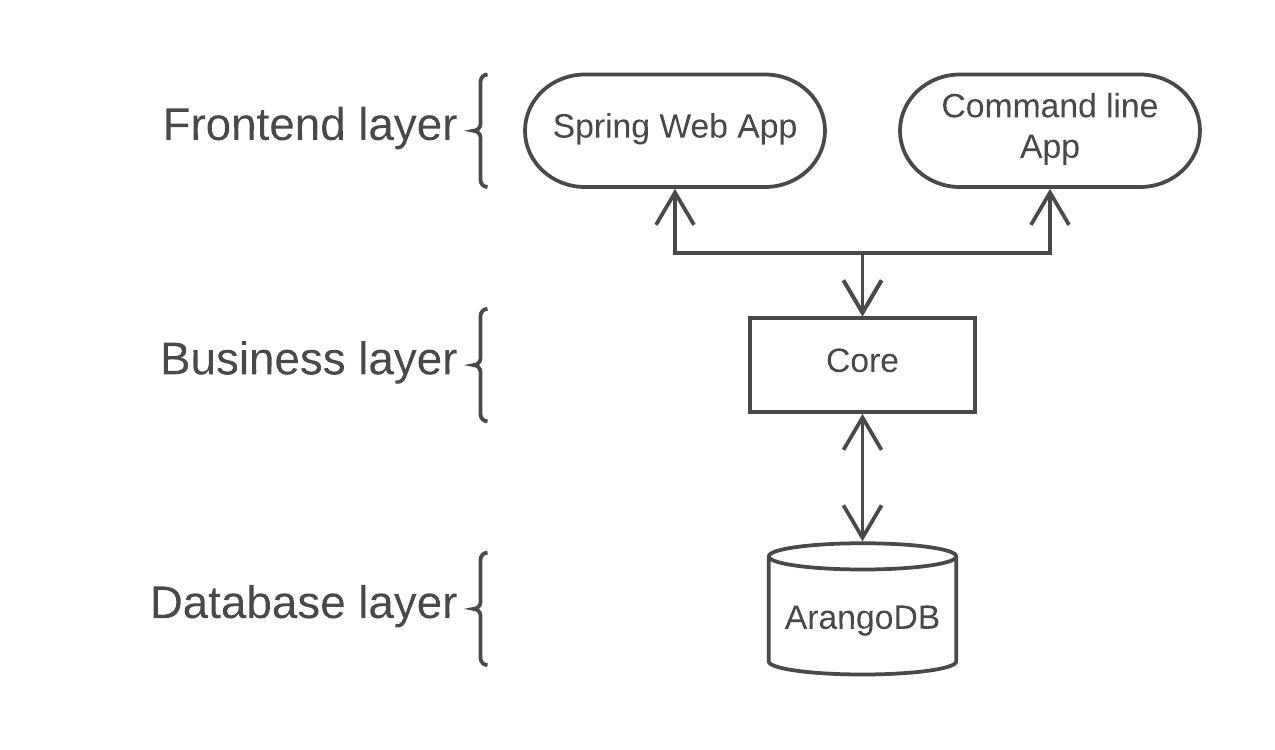
\includegraphics[width=300pt]{appdesign}
	\caption{\label{fig:appdesign} Structure of the app}
\end{figure}

\subsection{ArangoDB}

ArangoDB is a multi-model database. It supports three data models namely key/value, documents, graphs and a unified query language called AQL. AQL is very similar to SQL query language. AQL is used for CRUD operations. It provides scalabe and highly efficient queries. It uses JSON as a default storage schema. 

The application uses this database for all the heavy duty data operations like grouping, summing, filtering neighbours etc. The reason a database was used instead of doing it directly in Java was for faster development, thread-safety and also the indexes provided by the database for faster queries. 

\subsection{Core}

This business layer of the application contains all the core logic. It contains all the query, the driver to talk to ArangoDB, the logic for converting from and to csv etc. The core module uses spring-context which is an application IoC (Inversion of Control) container. This container can be consumed by any application by adding the library and providing the database connection configuration. This saves the other application from creating each and every object. The IoC container creates the object for the application automatically at runtime. The strategy was to create a library which contains all main logic and which can be consumed by any kind of application. This can be seen as we have implemented in two applications command line and web application.

Apart from using IoC containers, the main design pattern used by this module of application is the Command Pattern\cite{dupire2001command}. In this pattern, an object is encapsulated with all the information needed to perform an action. The biggest feature of the command pattern is that it can be executed at any point in time. The command in our case is executed by a Command executor. This separation of the actual command and executor allows for greater changes in the future of the project. It provides a lot of flexibility and ease of adding and replacing commands in later stages of the development. One of the purposes of using command pattern was the certain routines in the application are quite slow e.g. distance based clustering. The command pattern creates a unified way for getting the updates/progress of a task being executed.

The drawbacks of this pattern is it makes the source code larger quickly because one file can only represent one command. The number of files in the project increases very quickly. Command names are usually big and so goes for the file names. The order of commands becomes important at later stages and can jeopardize the reliability of the system\cite{dupire2001command}.

\begin{figure}[!ht]
	\centering
	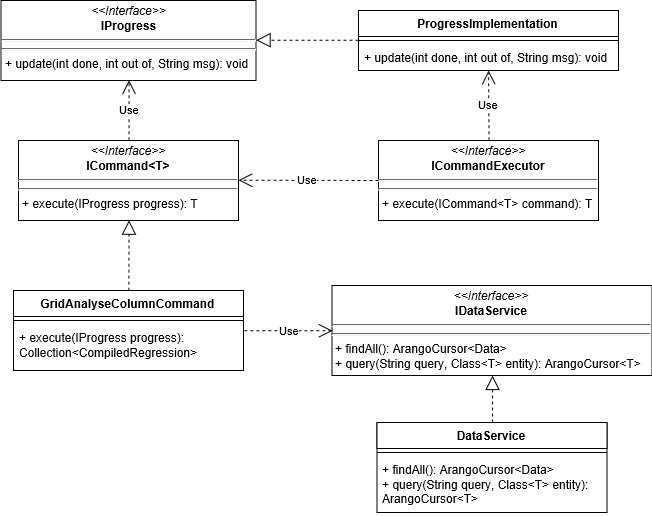
\includegraphics[width=300pt]{umlcore}
	\caption{\label{fig:umlcore} UML diagram of the command pattern in the core module}
\end{figure}

Figure\ref{fig:umlcore}, shows the implementation of command pattern. Only one Concrete command (GridAnalyseColumnCommand) is been shown. There are various commands implemented for data insertion, data deletion, distance based analysing etc. It can be seen from the figure\ref{fig:umlcore} that no implementation is defined for ICommandExecutor. This is because the modules consuming this core module library can implement according to their need. Similarly for the IProgress, modules can implement their own version depending on their type of the application. The parameters of the command are supplied when creating the instance of the object. The command object constructor contains all the necessary arguments needs for execution at later stage.

\subsection{Webapp}

The web application is built on Spring framework. It comes with IoC container which can easily pass in the database connection to the core library being consumed. In this module, the progress and command executor interfaces are implements to the needs of the web application. The progress interface implementation uses WebSocket for sending the update of how much work has been completed by the command. WebSocket is  full-duplex communication channel over TCP which allows server and client to send messages to each other asynchronously.

The application maps the REST APIs to the Commands in the core module. The UI of the web application uses AngularJS which is a client side front end web framework. AngularJS framework allows to makes calls to the REST Endpoints and also act accordingly to the messages received by the server through WebSocket.

\subsection{Command Line}

The command line application also uses the core module to do similar task. The mapping is from command line arguments to core module's command. In this module, as well a different implementation is done for the progress and command executor interfaces as this time the diplay and execution is in commandline. Since the core module uses IoC container. Spring-context was added and application context was created at the start of the applicaton. The arguments were parsed via the JCommander library. 

\section{Optimizations}

In this section, we discuss Optimizations that were done to speed up the computations.

\subsection{Grid clustering algorithm}

As per the pseudocode\ref{alg:gridExistence}, it can be seen that the Time complexity is \(O(N\log(N)\) which was due to the sorting performed on the coordinate of the box calculated for each data point. But as one can see from the pseudocode the two \(N\) iterations were performed. First for calculating the coordinate of the \(k-cube\) they belong to and then for the grouping the datapoints into the result. This result is then used for either finding violation of functional relation or for analysing the relation between the parameters. 

The two extra \(N\) iterations were optimised by the ArangoDB by dividing the 3 iterations into 2 nodes. First node sorted the data points by calculating the coordinates of the \(k-cube\) on the go and attaching it temporarily to the dataset for reuse if the data set is accessed again by the sort. After sorting the datapoints with its coordinates are send to the second node. The second node then groups the data on the fly as the groups are accessed. This is because the all the groups with equal coordinate lies next to each other. The groups and the data coming from the second node is pipelined to our computations that are performed on the nodes. 

It is impossible to parallelize this algorithm because of its aggregating nature, where one point cannot be in more than one cluster. But due to its \(O(N\log(N))\) complexity, overall the algorithm is quite fast and linear.

\subsection{Distance based clustering}

In the distance based clustering\ref{alg:dbscanExistence}, we calculated the time complexity to be \(O(N^2\). This was due to nature of the algorithm to find neighbouring data points for every data point in the dataset. 

It is not possible to reduce the first outer iteration, as we have to go through each data point for analysing the whole dataset. The second one, it is not required to go through the entire data points as long as we can find all the points that are close to each other within some tolerance. This makes it possible for optimisations. One of the approaches is to save \(N^2\) distances between each and every data point and then making it easier for all the subsequent queries. This is very practical and blazingly fast as only one time slow operation is required for saving all the distances between each and every point. Then finding neighbours is a trivial task of going through the entire edges and getting all those points where the distance is less than the specified tolerance. This is practical for smaller dataset but due to the square space complexity. But as the number of records get larger it becomes in efficient to not only run the one time insertion but also storing the same.

So, another way was chosen in which indexes were created to fasten the search to find the neighbours. We filter the data with conditions such that data points whose possibility of becoming neighbour is zero is filtered before the distance is actually and calculate and confirmed.

We use the fact that \(dist(v, u) \geq 0\) always where \(v, u\) are two data points vectors in space. 

Let the \(tol\) be the max distance (tolerance) allowed between two data points. 
Let \(u\) be the data point vector with dimension \(k\) whose neighbours are to be found.
Let \(v\) be any vector in the dataset.

Then for any value of:
\[v[i] > u[i] + tol \vee v[i] < u[i] - tol\] where \(i \in [0, k-1]\)
\[\implies dist(u, v) > tol\]

The reason is if any one of the values in vector \(v\) is more than \(tol\) units away then because the distance is added from all the other values of the vector as well. The total distance will definitely be more than \(tol\).

But this filtering method is still not good as we still have to go through all the dataset to check whether any of the value is greater than \(tol\) or not. ArangoDB provides APIs to create indexes on the fields of documents for faster access to documents. It provides many different types of indexes such as Hash index, skip list index, full text index etc. Each index uses a special data structure to fasten different types of searches. As we are interested in range based queries. Skip list comes into play. Skiplist maintains a separate linked heirarchy of ordered values. They fasten up the equality lookups, range queries and sorting. The skiplist is added on to every parameter of the dataset and then when the filtering out condition is used before calculating the distance. The number of iteration will drop from \(N\) to the \(Amortised-N\).

Another performance improvement that is done is by parallelising the outer loops. As ArangoDB supports multiple reads at the same time and the inner loop has no dependency on other iteration. Outer loop is parallelised which further decreases the running time by the number of threads the CPU can handle at a time. 


\chapter{Results and Evaluation}
When the task is to find the existence of functional relation, Data points which violates the functional relation definition are returned. If there are no such data points no records are returned. But when we move on to next step of analysing the functional relation a number of variables describing the clusters formed for analysing a particular parameter variable is returned. Following is the list of those variables.

\begin{itemize}
    \item \textit{Parameter nos}: index of the parameter that the analyses is ran for.
    \item \textit{Tolerance}: the tolerance which was given as input to be used for the clustering algorithm.
    \item \textit{Slope of the regression line}: mean and standard deviation of the slope from all the clusters formed.
    \item \textit{Y-intercept of the regression line}: mean and standard deviation of the y-intercept from all the clusters.
    \item \textit{Weighted slope and y-intercept}: Since finding a regression line requires only minimum 2 points. A number of small clusters can hide the values of the dense clusters. Weighted slope and y-intercept multiplies the values with the number of points in the data cluster to give more weightage to the dense clusters.
    \item \textit{Pearson correlation coefficient}: It is the measure of the linear correlation between two variables X and Y. It ranges from -1 to 1 represent total negative correlation to total positive correlation.
    \item \textit{\(R^2\)}: it is coefficient of determination explaining how good is the regression line fit.
    \item \textit{Number of outliers}: these are the numbers of clusters formed with only 1 data point.
    \item \textit{Number of cluster}: this represents the number of clusters formed with greater than 1 data member.
    \item \textit{Number of data points in each cluster}: average and standard deviation of number of data points in each cluster is returned
    \item Number of points that failed to provide a linear regression line: there are times when the linear regression cannot be calculated because the data points in the cluster have equal non clustered parameter variable values.

\end{itemize}

\section{Results}

The software was run on computer generated linear dataset as well as the real life experimental dataset. And for computer generated records. We found that the value of the \(constants\) used in generation of the records was equivalent to the mean of the \(slope\) computed from all the clusters formed with the accuracy of 10\%. The accuracy increased if the \(constants\) were larger and decreased if the \(constants\) were smaller. This was because it is easy to see the change when the parameter's contribution to the output is large. The \textit{standard deviation of the slope} was low when the function was linear. If any of the parameters contribution was non linear e.g. polynomial, the \textit{standard deviation of the slope} increased significantly. \textit{Weighted values} always had higher accuracy than the non weighted values.

The software requires an argument namely tolerance which is used as threshold for clustering. Below Figure \ref{fig:linegraph} shows the mean of Pearson coefficient R when the tolerance is increased form 0\% to 12\% for the experimental small dataset provided for the parameter number 4. Pearson coefficient is the measure of linear correlation. It tell how strong is the correlation between two variables. It can be seen in the graph for very low tolerance the Pearson coefficient is unreliable. This is because not many clusters are formed properly yet. As soon as the tolerance is increased. The correlation value increase substantially and reaches a maximum point for certain tolerance. After that, further increase in tolerance degrades the correlation. This is because non-neighbour points also get clustered due to the tolerance factor.

\begin{figure}[!ht]
	\centering
	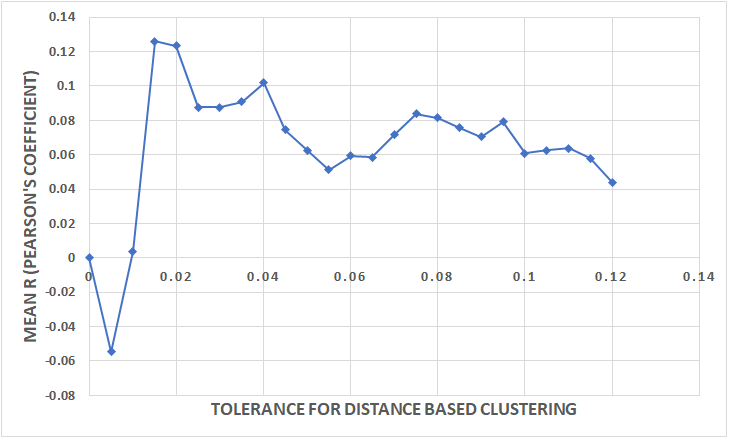
\includegraphics[width=400pt]{linegraph}
	\caption{\label{fig:linegraph} Pearson Coefficient vs Tolerance}
\end{figure}

\section{Challenges}

One of the challenges that was face while doing the analysis of the dataset was when the points are too far away from each other, this was because the units of one of the variable was really large. Since the parameter variable units were not comparable. The clustering algorithm was failing. Hence, to make it comparable the data was normalized. This normalization helped in making the parameters comparable. The tolerance was adjusted accordingly.

Another challenge faced was that because of normalization the real value of the slope got hidden. The normalization used was feature scaling the scales were changed and hence the slope and other values of the dataset didnot correspond to what they should. To solve this problem, the dataset was then clustered using normalized value but the regression line was created for the raw values of the dataset. This help solve the clustering as well as the regression problem.


\chapter{Conclusions and Future Work}
\section{Conclusion}

In this project, a successful software was created which enabled the ability to understand the relation between input parameter variable and the output variable. The software was run on experimental data set where the input parameters and the output variable corresponds to the performance events and the energy consumption. The software enabled us to cluster the data with various tolerance and analyse the effect of tolerance. This also helps in understanding and finding the optimum tolerance in the dataset where the functional relation is linear the most. It can be used for validating the linear models already in place and understand the relationship between variables on a much higher level.

The project has certain limitation such as the presence of a non-influential performance event or parameter could lead inaccurate result. The software works well with noise as the first step of the existence of functional relation could stop the noise from the analysis. But the addition of noise variable would corrupt the results significantly. Another limitation of the project is that it can only verify linear models and can only analyse linear relation.

\section{Future work}

More work is needed in the clustering algorithm because the Euclidean distance is not always the right choice for finding the difference between two points. As per\cite{aggarwal2001surprising}, the Euclidean distance measure does not work accurately because of the effect of the curse of high dimensionality.

The regression analysis right now is only linear. We would want to be able to analyse and validate other models such as \(\log\), polynomial etc. Each cluster must go through different regression analysis and pick the model which best fits the dataset.

%%%% ADD YOUR BIBLIOGRAPHY HERE
\newpage

\bibliography{references}
\bibliographystyle{plain}\label{endpage}

\appendix
\chapter{}
Project repository link:
\url{https://github.com/Sukrat/FYP2017-function-relationship-finder}



\end{document}
